\documentclass{article}
\usepackage[spanish]{babel}
\usepackage[utf8]{inputenc}
\usepackage{listings}
\usepackage[left=3cm,right=3cm,top=2cm,bottom=2cm]{geometry}
\usepackage{amsmath}
\usepackage[document]{ragged2e}
\usepackage{color}
\usepackage{graphicx}
\usepackage{hyperref}
\usepackage{float}

\hypersetup{
    colorlinks=true,
    linkcolor=blue,
    urlcolor=blue,
}

\definecolor{background}{RGB}{246,246,246}

\lstset{ %
  %backgroundcolor=\color{background},
  language=c++,
  directivestyle={\color{black}}
}

\begin{document}

\title{\Huge ED - Reto 4}
\author{\Large Javier Gálvez Obispo}
\date{\large\today}
\maketitle

\begin{flushleft}
  {\Large Dar un procedimiento para guardar un árbol binario en disco de forma que se
  recupere la estructura jerárquica de forma unívoca usando el mínimo número
  de centinelas que posible.}


  \vspace{\baselineskip}
  Como ejemplo usaremos el siguiente árbol binario generado aleatoriamente en esta
  \href{http://btv.melezinek.cz/binary-search-tree.html}{página}
\end{flushleft}

\begin{figure}[H]
  \centering
  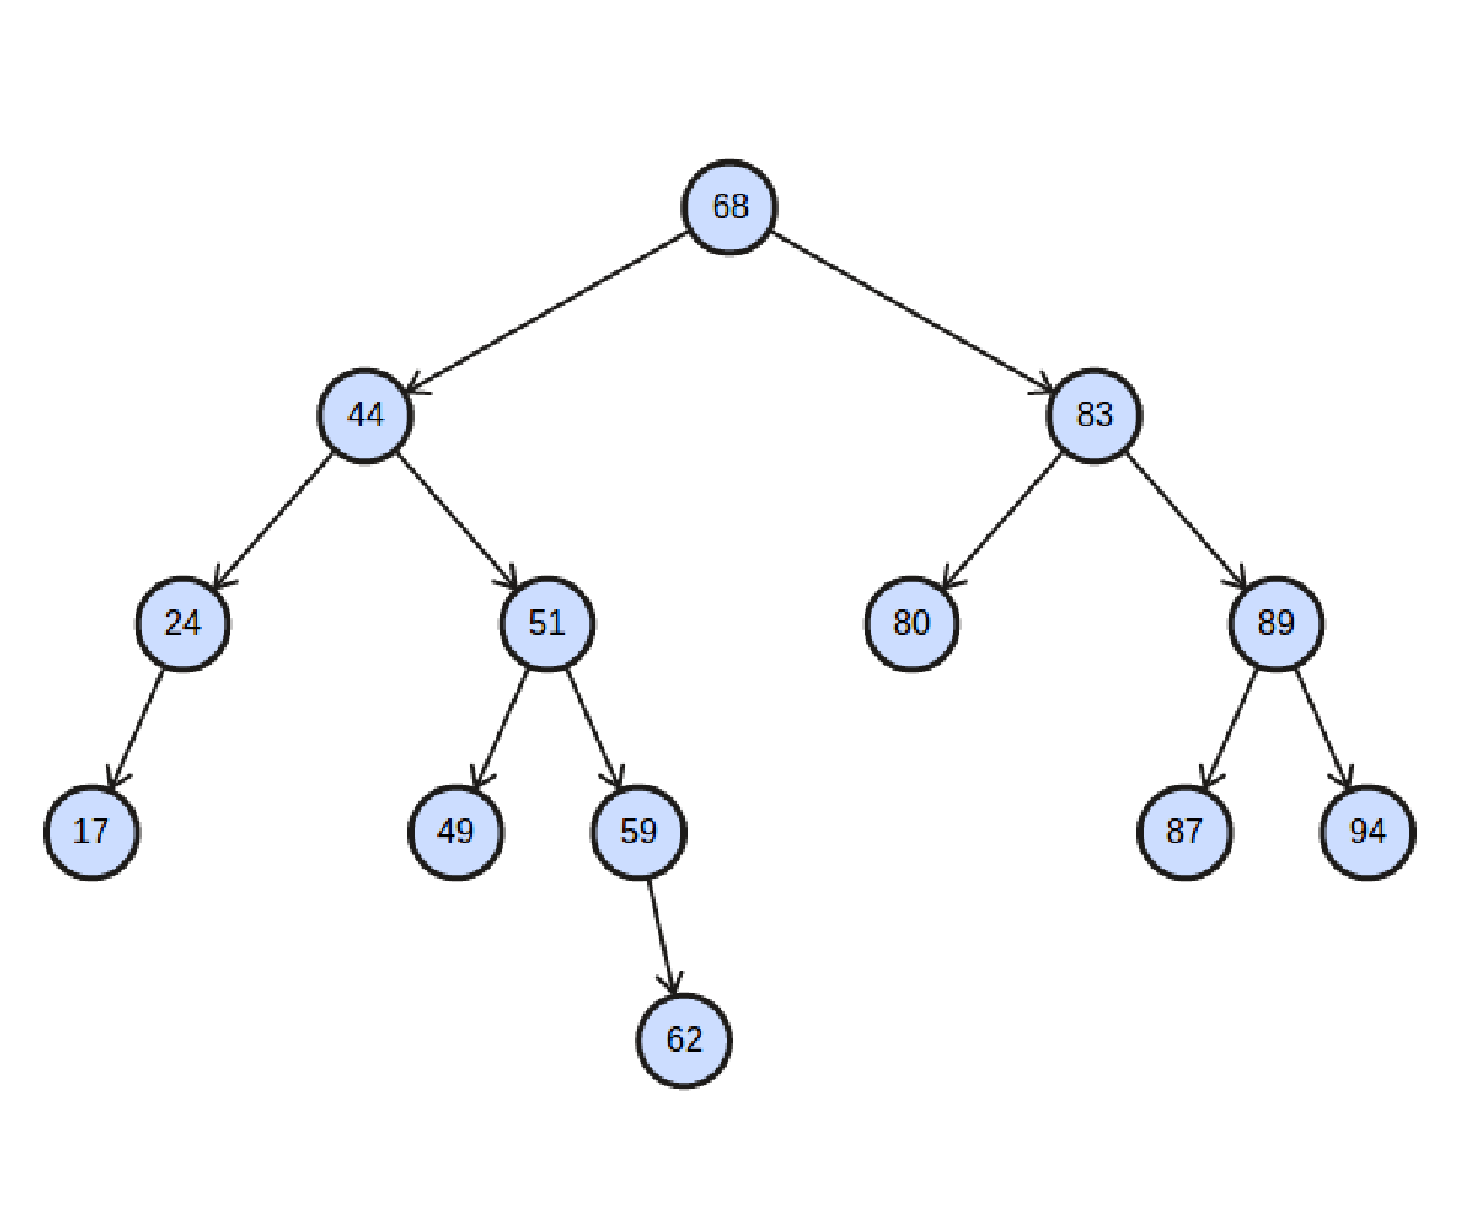
\includegraphics[width=\textwidth,height=\textheight,keepaspectratio]{arbol.eps}
  \caption{Arbol binario.}
\end{figure}

\newpage
\begin{flushleft}
  Primero definiremos el tipo \textbf{Byte} como un \textbf{unsigned char}
  \begin{lstlisting}
    typedef unsigned char Byte;
  \end{lstlisting}
  Esto lo hacemos ya que vamos a utilizar bytes como centinelas, es decir, cada bit
  del centinela significará si el nodo al que corresponde tiene un hijo a su izquierda o
  derecha dependiendo del caso.

  Por ejemplo, utilizando el árbol que hemos generado, los bits de la raíz serían 11 mientras que los
  bits del nodo con valor 24 serían 10 o los del nodo 62 que serían 00.
  Por cada centinela que utilicemos podremos guardar información de hasta 4 nodos.

  \vspace{\baselineskip}
  Para que no haya ambigüedad guardaremos la información de los nodos por niveles empezando por los
  que se encuentras más a la izquierda, activando primero los bits más significativos del byte.
  En nuestro caso el primer centinela almacenaría la información de los nodos 68, 44, 83 y 24.
  Al nodo 68 le corresponden los 2 bits más significativos y los dos estarían encendidos,
  al nodo 44 los 2 siguientes y así hasta llegar al último nodo. \vspace{\baselineskip}

  Entonces la representación de los centinelas de nuestro árbol binario queda así:
  \begin{lstlisting}
    Primer centinela:  11111110
    Segundo centinela: 11001100
    Tercer centinela:  00010000
    Cuarto centinela:  00000000
  \end{lstlisting}

  Pero en esta representación estamos utilizando 4 bytes (16 nodos) y tenemos sólo 13 nodos.
  Estamos desperdiciando 6 bits de un centinela, realmente no es tan grande la pérdida que tenemos.

  \vspace{\baselineskip}
  La ventaja de haber definido nuestro tipo \textbf{Byte} como \textbf{unsigned char} la encontramos al guardar los centinelas
  en un archivo. Aunque nosotros los utilizemos como bytes no hay que olvidar que son del tipo \textbf{unsigned char}
  y por tanto podemos almacenarlos en un fichero como tal en vez de usar la representación de antes.
  \vspace{\baselineskip}

  Así que a la hora de almacenar el árbol en un fichero primero tendríamos una línea con todos los centinelas
  y en la segunda línea tendríamos las etiquetas de los nodos. \break
  Para leer el fichero primero guardaríamos en un vector los centinelas leyéndolos uno a uno
  hasta llegar al final, y una vez leídos todos, guardaríamos las etiquetas en otro vector. \break
  Reconstruir el árbol sería sencillo ya que tenemos tanto los centinelas como las etiquetas almacenados por
  niveles y sabemos la estructura que tiene el árbol.

  \vspace{\baselineskip}
  Con esto conseguimos reducir el número de datos almacenados a:
    $$ n + f(n/4) $$
  siendo n el número de etiquetas y f la función parte entera. Si n es divisible entre 4,
  en caso contrario tendríamos que sumar 1 al resultado. \break
  En nuestro caso concreto tenemos:
    $$ datos = 13 + f(13/4) + 1 = 14 + 3 = 17 $$
  y efectivamente tenemos 13 etiquetas y 4 centinelas dando un total de 17 datos mientras que
  de la forma usual de almacenar árboles binarios tendríamos 27.
\end{flushleft}

\end{document}
